\makeatletter\let\ifGm@compatii\relax\makeatother
\documentclass[pdf, 10pt]{beamer}
\mode<presentation>{\usetheme{Warsaw}}
\usepackage{listings}
\usepackage{relsize}

%% https://tex.stackexchange.com/questions/4302/prettiest-way-to-typeset-c-cplusplus
%% \newcommand\CC{C\nolinebreak\hspace{-.05em}\raisebox{.4ex}{\relsize{-3}{\textbf{+}}}\nolinebreak\hspace{-.10em}\raisebox{.4ex}{\relsize{-3}{\textbf{+}}}}
\protected\def\CC{C\nolinebreak[4]\hspace{-.05em}\raisebox{.4ex}{\relsize{-3}{\bf ++}}\,}

%% preamble
\title{EMF4CPP}
\subtitle{Generating Ecore Models for \CC}
\author[Matthias D\"orfel]{Matthias D\"orfel, INCHRON GmbH\\
  \href{mailto:doerfel@inchron.com}{doerfel@inchron.com}}
\date{MUC\nolinebreak[4]\hspace{-.05em}\raisebox{.4ex}{\relsize{-3}{\bf ++}}\\ September 19, 2018}




\begin{document}


%%%%%%%%%%%%%%%%%%%%%%%%
%% title frame
\begin{frame}
\titlepage
\end{frame}
%%%%%%%%%%%%%%%%%%%%%%%%


\begin{frame}{Overview}
  \begin{itemize}
  \item EMF4CPP allows to use the Eclipse Modeling Framework in \CC projects
  \item Reuse metamodels based on ecore
  \item Generate a \CC class hierarchy
  \item Runtime support system with generic algorithms based on reflection
  \item Exchange of model instances serialized as XMI
  \end{itemize}
\end{frame}
%%%%%%%%%%%%%%%%%%%%%%%%

\section{Models}

\subsection{\CC}

\defverbatim[colored]\lstCppModel{
\begin{lstlisting}[language=C++,basicstyle=\ttfamily,keywordstyle=\color{blue}]
auto d = new Department;
p->getEmployees().push_back(new Employee);
\end{lstlisting}
}

\begin{frame}{Models, Metamodels and Meta-Metamodels}
A model (or model instance) is formed by objects at runtime
\lstCppModel

\end{frame}
%%%%%%%%%%%%%%%%%%%%%%%%

\defverbatim[colored]\lstCppMetaModel{
\begin{lstlisting}[language=C++,basicstyle=\ttfamily,keywordstyle=\color{blue}]
class Employee;
class Department {
    Employee* m_manager = nullptr;
    std::vector<Employee*> m_employees;
public:
    Department() = default;

    Employee* getManager() { return m_manager; }
    void setManager(Employee* e) { m_manager = e; }

    std::vector<Employee*>& getEmployees() { 
        return m_employees; }
};
\end{lstlisting}
}

\begin{frame}{Models, Metamodels and Meta-Metamodels}
The metamodel is the class definition
\lstCppMetaModel

\end{frame}
%%%%%%%%%%%%%%%%%%%%%%%%

\subsection{Ecore}

\begin{frame}{Models, Metamodels and Meta-Metamodels}
The metamodel is the class definition
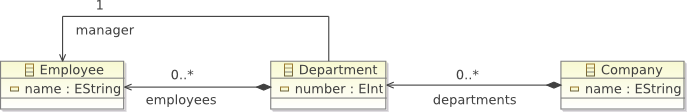
\includegraphics[width=\textwidth]{company-metamodel.png}
\end{frame}
%%%%%%%%%%%%%%%%%%%%%%%%

\subsection{Ecore Metamodel}

\begin{frame}{Models, Metamodels and Meta-Metamodels}
The metamodel is an instance of the Ecore model
\begin{center}
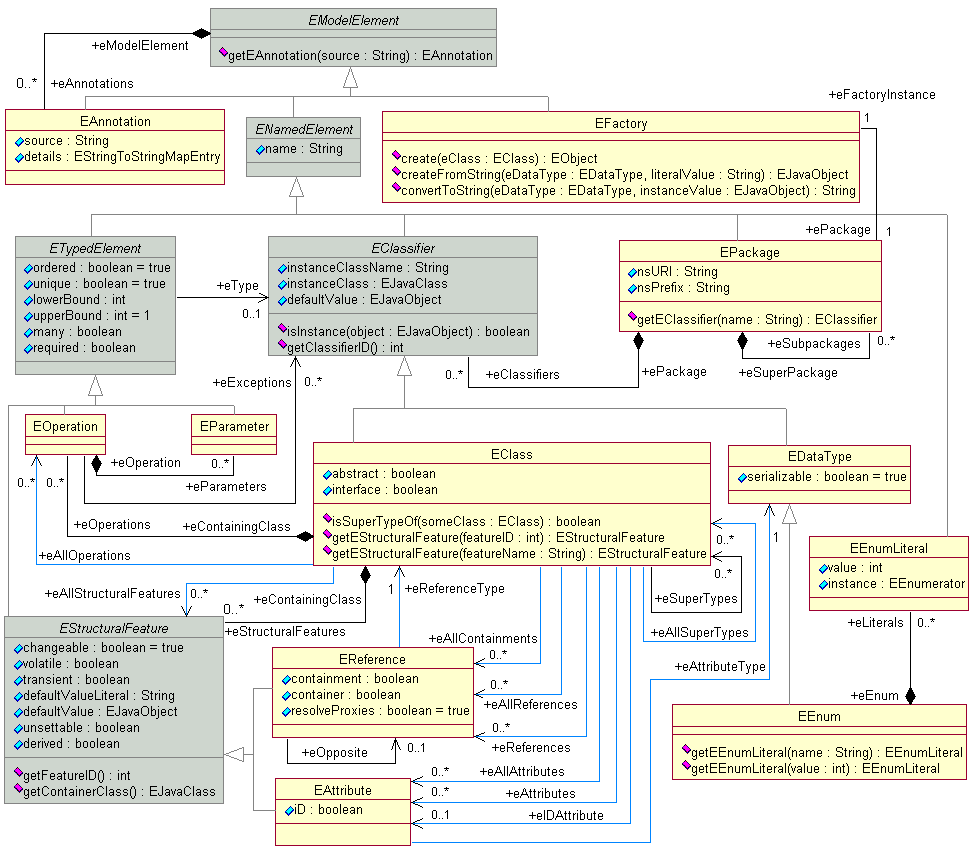
\includegraphics[width=\linewidth,height=0.8\textheight,keepaspectratio]{EMF/EcoreRelations.png}
\end{center}
\end{frame}
%%%%%%%%%%%%%%%%%%%%%%%%

\begin{frame}{Models, Metamodels and Meta-Metamodels}
At the core: EClass
\begin{center}
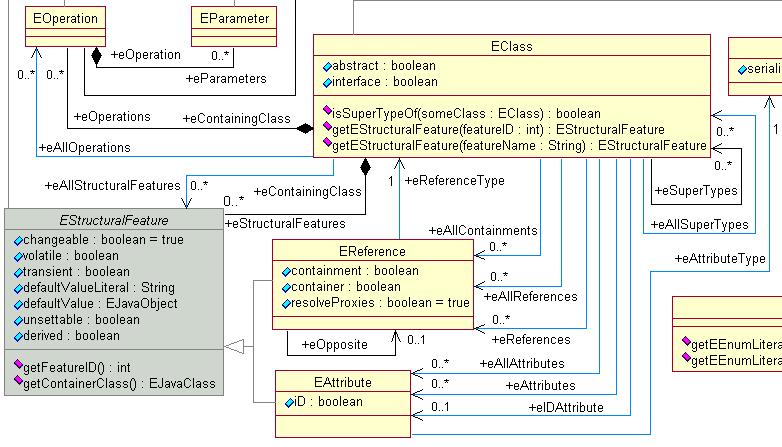
\includegraphics[width=\linewidth,height=0.8\textheight,keepaspectratio]{EMF/EcoreRelations-EClass.png}
\end{center}
\end{frame}
%%%%%%%%%%%%%%%%%%%%%%%%

\begin{frame}{Models, Metamodels and Meta-Metamodels}
At the core: EClass
\begin{center}
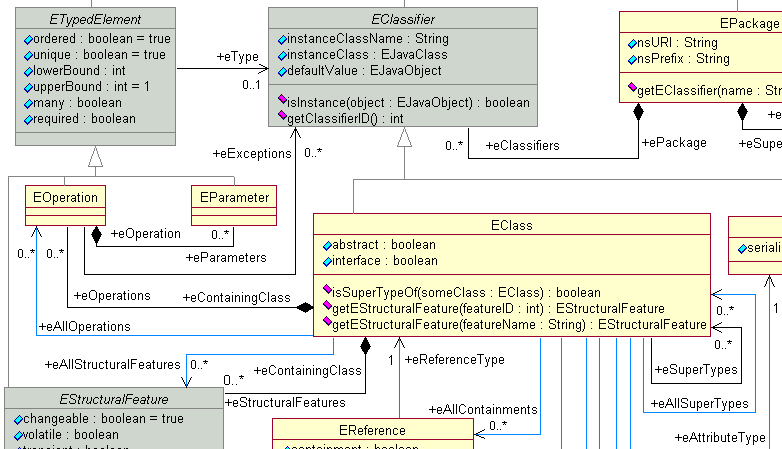
\includegraphics[width=\linewidth,height=0.8\textheight,keepaspectratio]{EMF/EcoreRelations-ETypedElement.png}
\end{center}
\end{frame}
%%%%%%%%%%%%%%%%%%%%%%%%


\section{EMF4CPP}

\subsection{Usage}

\begin{frame}{Usage}
\center{
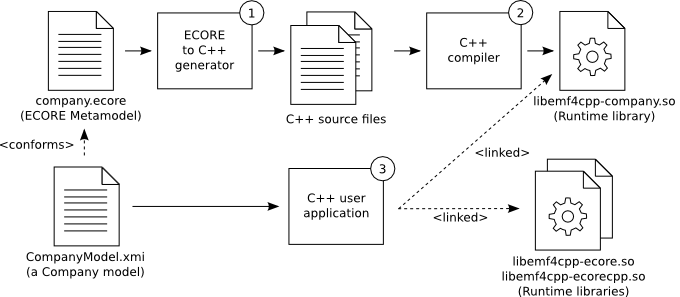
\includegraphics[width=\linewidth,height=0.8\textheight,keepaspectratio]{company-workflow.png}}
\end{frame}
%%%%%%%%%%%%%%%%%%%%%%%%

\subsection{Codegeneration Strategy}

\begin{frame}{Codegeneration Strategy}
  \begin{itemize}
  \item For each class in the ecore model, a \CC class is generated
  \item Objects are managed by boost::intrusive\_ptr$<>$
  \item Containers are based on std::vector$<>$
  \item Classes are PODs -- more or less
  \item<2-> Extend the generated code by
    \begin{itemize}
    \item {\em PROTECTED REGION}s are kept by the code generator
    \item Derive and instantiate your own classes by {\em factory injection}
    \end{itemize}
  \end{itemize}
\end{frame}
%%%%%%%%%%%%%%%%%%%%%%%%

\defverbatim[colored]\lstDepartment{
\begin{lstlisting}[language=C++,basicstyle=\ttfamily\scriptsize,keywordstyle=\color{blue},breaklines=true]
namespace company {

class Department : public virtual ::ecore::EObject {
public:
    Department();
    virtual ~Department();

    // Operations

    // Attributes
    virtual ::ecore::EInt getNumber () const;
    virtual void setNumber (::ecore::EInt _number);

    // References
    virtual const ::ecorecpp::mapping::EList< ::company::Employee_ptr >& getEmployees () const;
    virtual ::ecorecpp::mapping::EList< ::company::Employee_ptr >& getEmployees ();

    virtual ::company::Employee_ptr getManager () const;
    virtual void setManager (::company::Employee_ptr _manager);
\end{lstlisting}
}


\defverbatim[colored]\lstDepartmentx{
\begin{lstlisting}[language=C++,basicstyle=\ttfamily\scriptsize,keywordstyle=\color{blue},breaklines=true]
    /* This is the same value as getClassifierId() returns, but as a
     * static value it can be used in template expansions. */
    static const int classifierId = CompanyPackage::DEPARTMENT;

    /*PROTECTED REGION ID(Department) START*/
    // Please, enable the protected region if you add manually written code.
    // To do this, add the keyword ENABLED before START.
    /*PROTECTED REGION END*/

protected:
    // Attributes
    ::ecore::EInt m_number;

    // References
    std::shared_ptr<::ecorecpp::mapping::EList< ::company::Employee_ptr >> m_employees;
    ::company::Employee_ptr m_manager;
};

} //namespace Company
\end{lstlisting}
}

\begin{frame}{Codegeneration Strategy}
\lstDepartment
\end{frame}

\begin{frame}{Codegeneration Strategy}
\lstDepartmentx
\end{frame}

%%%%%%%%%%%%%%%%%%%%%%%%

\begin{frame}{Reference Handling}
  \begin{itemize}
  \item<1-> All references are handled as boost::intrusive\_ptr$<>$
  \item<1-> Multiplicity $>1$ implemented by spezialized container {\em EList}
  \item<1-> Opposite relation
    \begin{itemize}
    \item<2-> Changing a relation implicitly changes relation at referenced object
    \item<2-> Opposite relations can have different multiplicity
    \item<2-> Example: Employee is a manager for multiple Departments\\
      \lstinline[language=C++,basicstyle=\ttfamily,keywordstyle=\color{blue}]{Employee::getManagedDepartments()}
$\iff$
\lstinline[language=C++,basicstyle=\ttfamily,keywordstyle=\color{blue}]{Department::getManager()}
    \end{itemize}
  \item<1-> Containment relation
    \begin{itemize}
    \item<3-> Express ownership
    \item<3-> Implicit opposite relation: eContainer()
    \item<3-> Removing a child \textbf{must not} implicitly delete the child
    \end{itemize}
  \item<4-> Implemented by generated code in combination with EList container
  \end{itemize}
\end{frame}
%%%%%%%%%%%%%%%%%%%%%%%%

\subsection{Runtime Support System}

\begin{frame}{libemf4cpp-ecorecpp}
  \begin{itemize}
  \item Serialization / deserialization as XML Metadata Interchange (XMI)
  \item Resources and ResourceSets
    \begin{itemize}
    \item Resources reference URIs, e.g. files
    \item Instances can be split over Resources
    \end{itemize}
  \item Tree traversal
  \item Notification framework
    \begin{itemize}
    \item Callbacks for modifications of the model
    \item Useful for Model-View-Controller UIs
    \end{itemize}
  \item<2-> Generic, model-agnostic implementation
  \end{itemize}
\end{frame}
%%%%%%%%%%%%%%%%%%%%%%%% 

\subsection{Reflection}

\begin{frame}{Reflection API}
  \begin{itemize}
  \item libemf4cpp-ecore
    \begin{itemize}
    \item \CC\,implementation of the ecore metamodel
    \item Created during bootstrap build of the codegenerator
    \end{itemize}
  \item Every generated class is derived from ecore::EObject
  \end{itemize}
\end{frame}
%%%%%%%%%%%%%%%%%%%%%%%%

\begin{frame}{Operations Defined for ecore::EObject}
\begin{center}
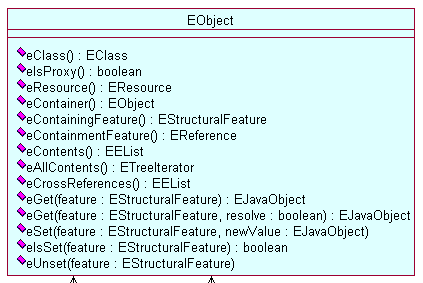
\includegraphics[width=\linewidth,height=0.8\textheight,keepaspectratio]{EMF/EObjectOperations-focused.png}
\end{center}
\end{frame}
%%%%%%%%%%%%%%%%%%%%%%%%

\begin{frame}{Know Your Metaclass}
  \begin{itemize}
  \item For each generated class, the runtime system initializes an instance
    of ecore::EClass
  \item Instances know their ecore::EClass: 
    \lstinline[language=C++,basicstyle=\ttfamily,keywordstyle=\color{blue}]{employee->eClass()}
  \item<2-> Examine the class definition by
    \begin{itemize}
    \item Class hierarchy: eSuperTypes(), eAllSuperTypes()
    \item Members: eStructuralFeatures(), eAllStructuralFeatures()\\
      as well as eAttributes(), eReferences(), ...
    \end{itemize}
  \item<3-> Access instances by generic APIs
    \begin{itemize}
    \item Access to members:\\eGet(someFeature), eSet(someFeature, newValue)
    \item The parent: eContainer(), eContainingFeature()
    \item All children: eContents(), eAllContents()
    \end{itemize}
  \end{itemize}
\end{frame}
%%%%%%%%%%%%%%%%%%%%%%%%

\section{Participation}

\subsection{Licensing}

\begin{frame}{Licensing: LGPL}
  \begin{itemize}
  \item The codegenerator, the runtime libraries and the generated
    ecore implementation: published under LGPL
  \item Code generated from an ecore model: It's yours!\\
    (Actually most lawyers think, it belongs to the owner of the model)
  \end{itemize}
\end{frame}
%%%%%%%%%%%%%%%%%%%%%%%%

\subsection{Github}

\begin{frame}{Project URL}
First release in 2010\\
Research project at University of Murcia, Spain\\
\href{https://github.com/catedrasaes-umu/emf4cpp}{https://github.com/catedrasaes-umu/emf4cpp}\\[1em]

Presented features are implemented in a fork\\
\href{https://github.com/mdoerfel/emf4cpp}{https://github.com/mdoerfel/emf4cpp}\\[1em]

Participation is welcome!\\[1em]
Contact me for questions: \href{mailto:doerfel@inchron.com}{doerfel@inchron.com}
\end{frame}
%%%%%%%%%%%%%%%%%%%%%%%%

%%%%%%%%%%%%%%%%%%%%%%%%
%%%%%%%%%%%%%%%%%%%%%%%%
%%%%%%%%%%%%%%%%%%%%%%%%




\end{document}
